


\subsection{Ablations on Modules}

% \begin{figure}[ht]
%      \centering
%      \begin{subfigure}{0.4\textwidth}
%          \centering
%          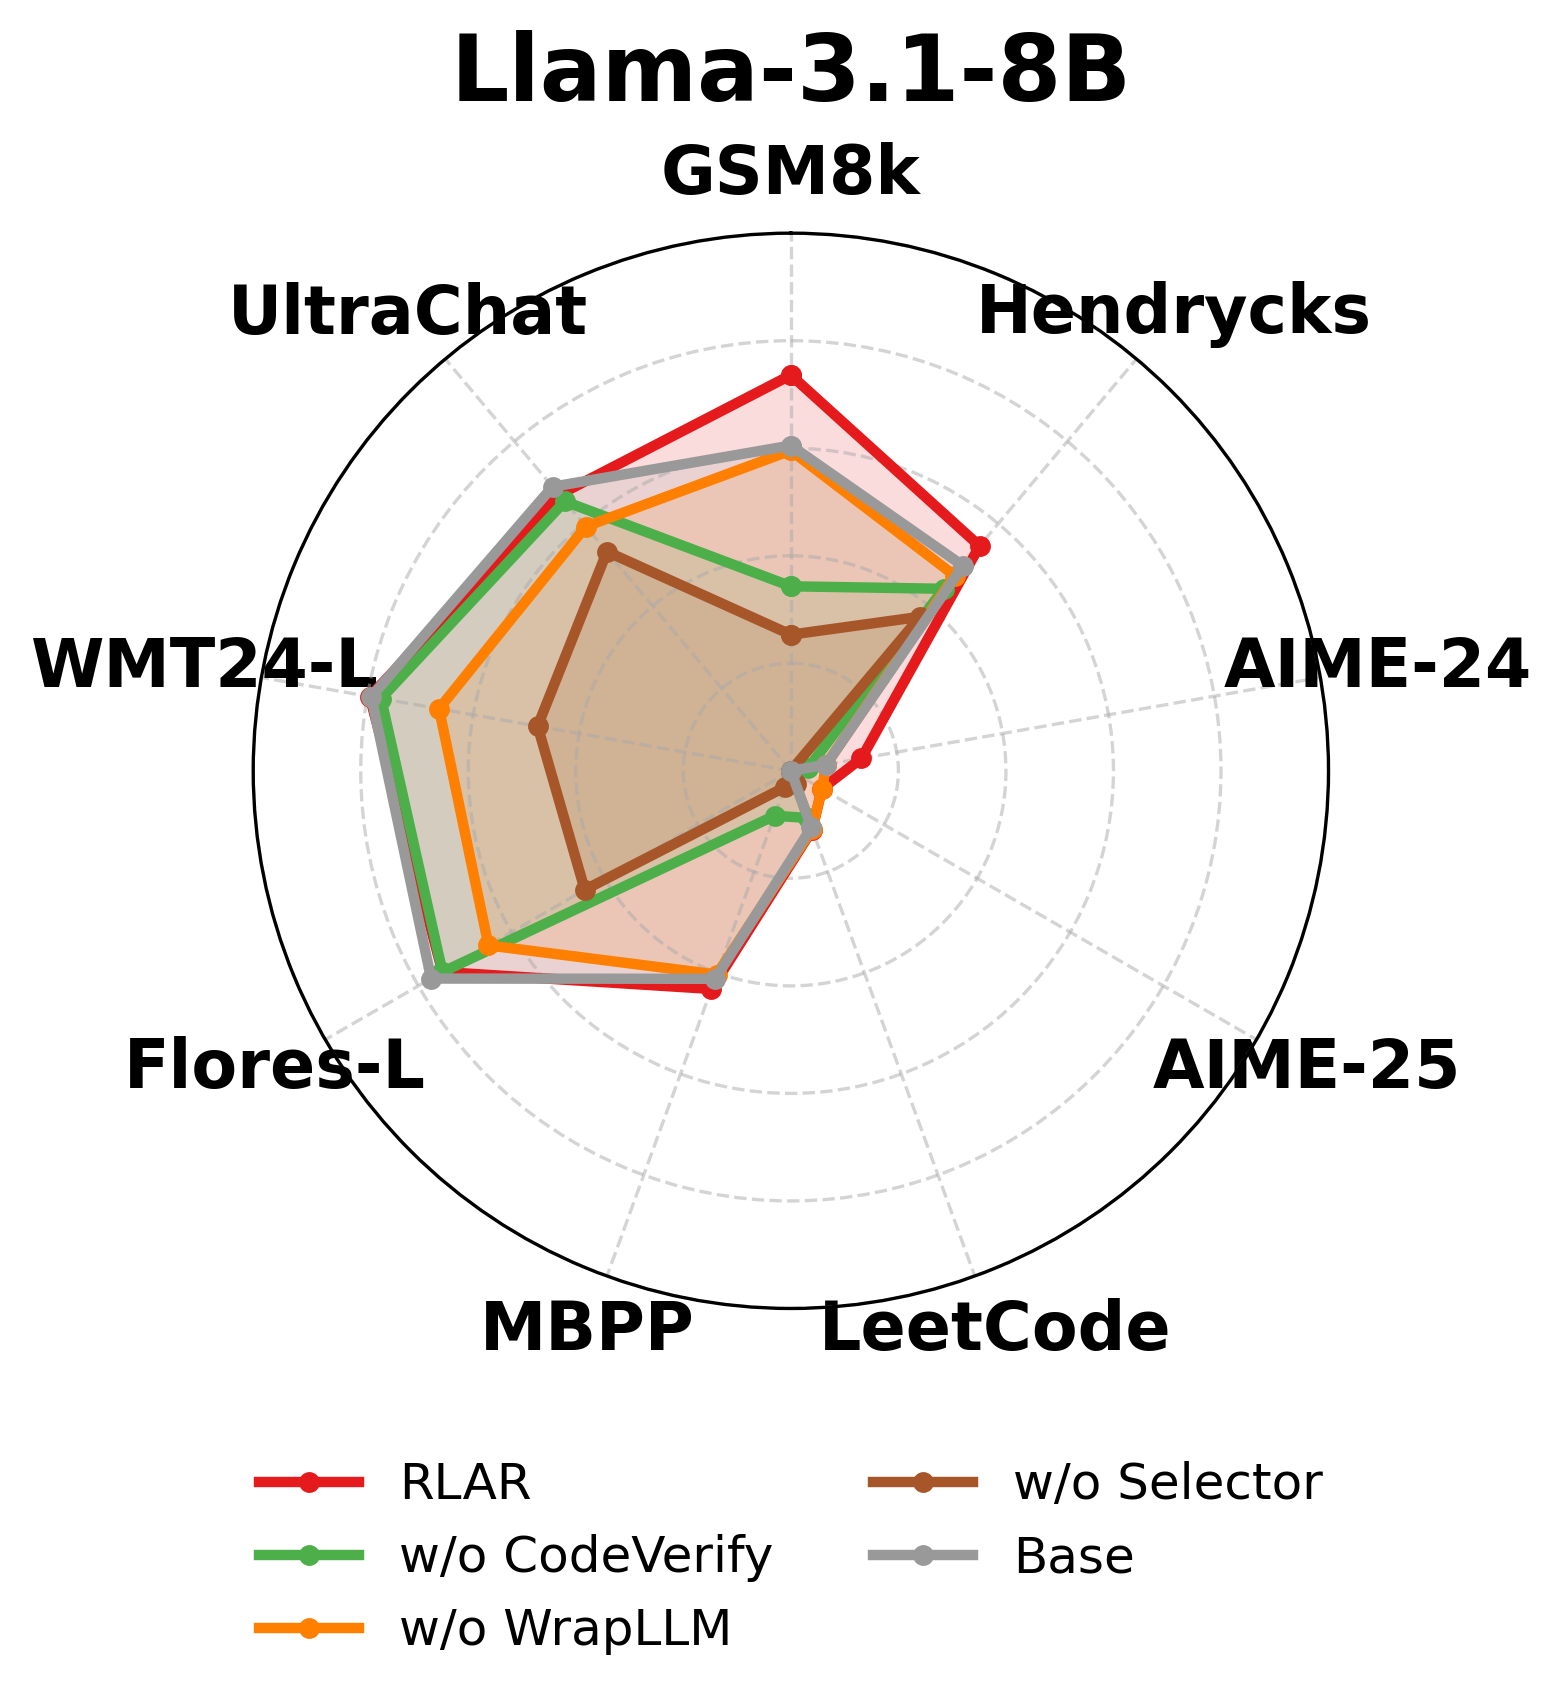
\includegraphics[width=0.8\linewidth]{Figures/llama_ablation.png}
%          \caption{Llama-3.1-8B}
%          \label{fig:abl_llama}
%      \end{subfigure}
%      \hfill
%      \begin{subfigure}{0.4\textwidth}
%          \centering
%          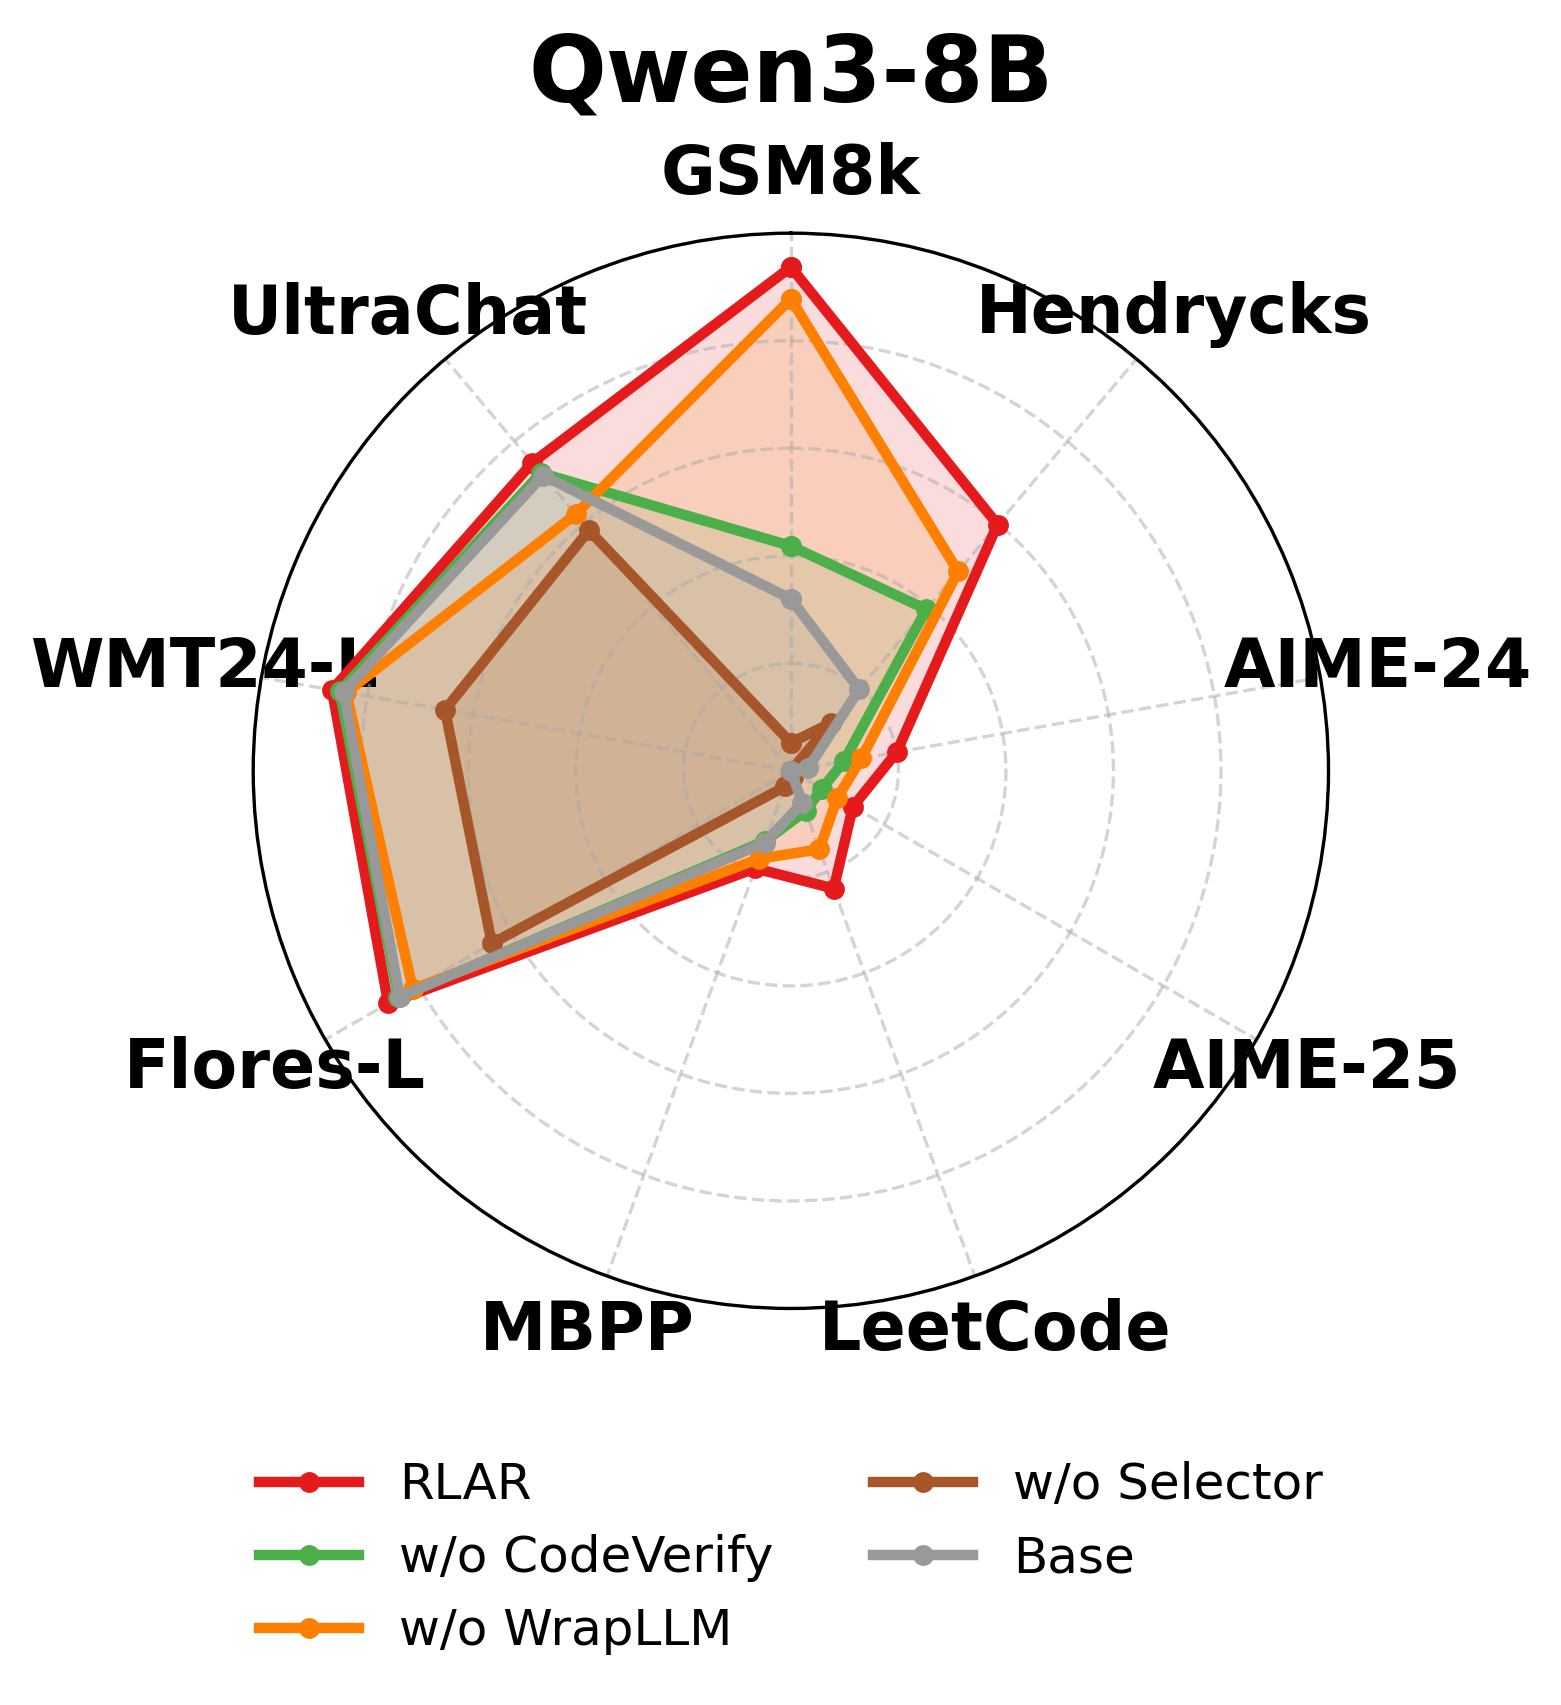
\includegraphics[width=0.8\linewidth]{Figures/qwen_ablation.png}
%          \caption{Qwen3-8B}
%          \label{fig:abl_qwen}
%      \end{subfigure}
%      \caption{Ablation studies on Llama-3.1 and Qwen3.}
%      \label{fig:ablation}
% \end{figure}

To investigate the contribution of each component within the \method{} framework, we conduct an ablation study with the following configurations: (1) \textbf{w/o CodeVerify} and (2) \textbf{w/o WrapLLM}, which respectively disable the corresponding actions in the tool synthesis module; and (3) \textbf{w/o Selector}, where instead of immediate selection post-synthesis, a reward tool is randomly sampled only after all reward tools have been generated. Results of these variants are shown in Figure~\ref{fig:ablation}.

Removing either component of the tool synthesis module consistently results in degradation. Specifically, \textbf{without CodeVerify}-designed tools, mathematical reasoning and coding tasks (\textsc{GSM8k, LeetCode}) drop significantly. \textbf{WrapLLM} is essential for chat and translation tasks. The above results confirm the necessity of query-specific reward designs, which is the core motivation of \method{}. 


Moreover, the Random Reward Selection variant (\textbf{w/o Selector}) underscores the importance of reward matching. The policy degrades on almost all benchmarks. This confirms that appropriate reward selection is crucial in the overall RL training procedure, and that our framework effectively synthesizes high-quality reward tools superior to random alternatives.



% We have further conducted the analysis on the WrapLLM search engine design. The average retrieved model repository position is 5.64 in the first page, showing the relatedness. \textbf{Further error analyses are included in Appendix}~\ref{sec:error_robustness}.

We further analyzed the WrapLLM search engine design. The average retrieved model position is 5.64 on the first page, indicating high relevance. \textbf{Error analyses are in Appendix}~\ref{sec:error_robustness}.

